\documentclass[a4paper,11pt]{report}-
\usepackage[utf8]{inputenc}
\usepackage[dutch]{babel}
\usepackage{geometry}
\usepackage{graphicx}
\usepackage{lmodern}
\usepackage{amsmath, amssymb}
\usepackage{pdfpages} 

\usepackage[T1]{fontenc}
\usepackage{longtable}
\usepackage{xcolor}
\usepackage{color}
\usepackage{fancyvrb}
\usepackage{lipsum}
\usepackage{setspace}
\usepackage{tocbibind}
\usepackage{array} 
\usepackage{multicol}
\usepackage{tikz}
\usetikzlibrary{arrows.meta,shapes.geometric, arrows, positioning}
\usepackage[hidelinks]{hyperref}
\usepackage{titlesec} 
\usepackage{algorithm}
\usepackage{amsfonts}
\usepackage{caption}
\usepackage{mathtools}
\usepackage{algpseudocode}
\usepackage{listings}
\usepackage[
backend=biber,
style=nature,
]{biblatex}
\addbibresource{references.bib}

\algrenewcommand{\alglinenumber}[1]{#1}

\setlength{\parskip}{0.8em}
\setlength{\parindent}{0pt}

\nocite{*}

\hypersetup{
    colorlinks=true,     % false: boxed links; true: colored links
    linkcolor=black,     % color of internal links
    citecolor=blue,      % color of citations
    urlcolor=blue        % color of external urls
}
\pagenumbering{Roman}  % Romeinse nummering

\geometry{a4paper, top=3.5cm, bottom=3.5cm, left=2.5cm, right=2.5cm} 

\begin{document} 

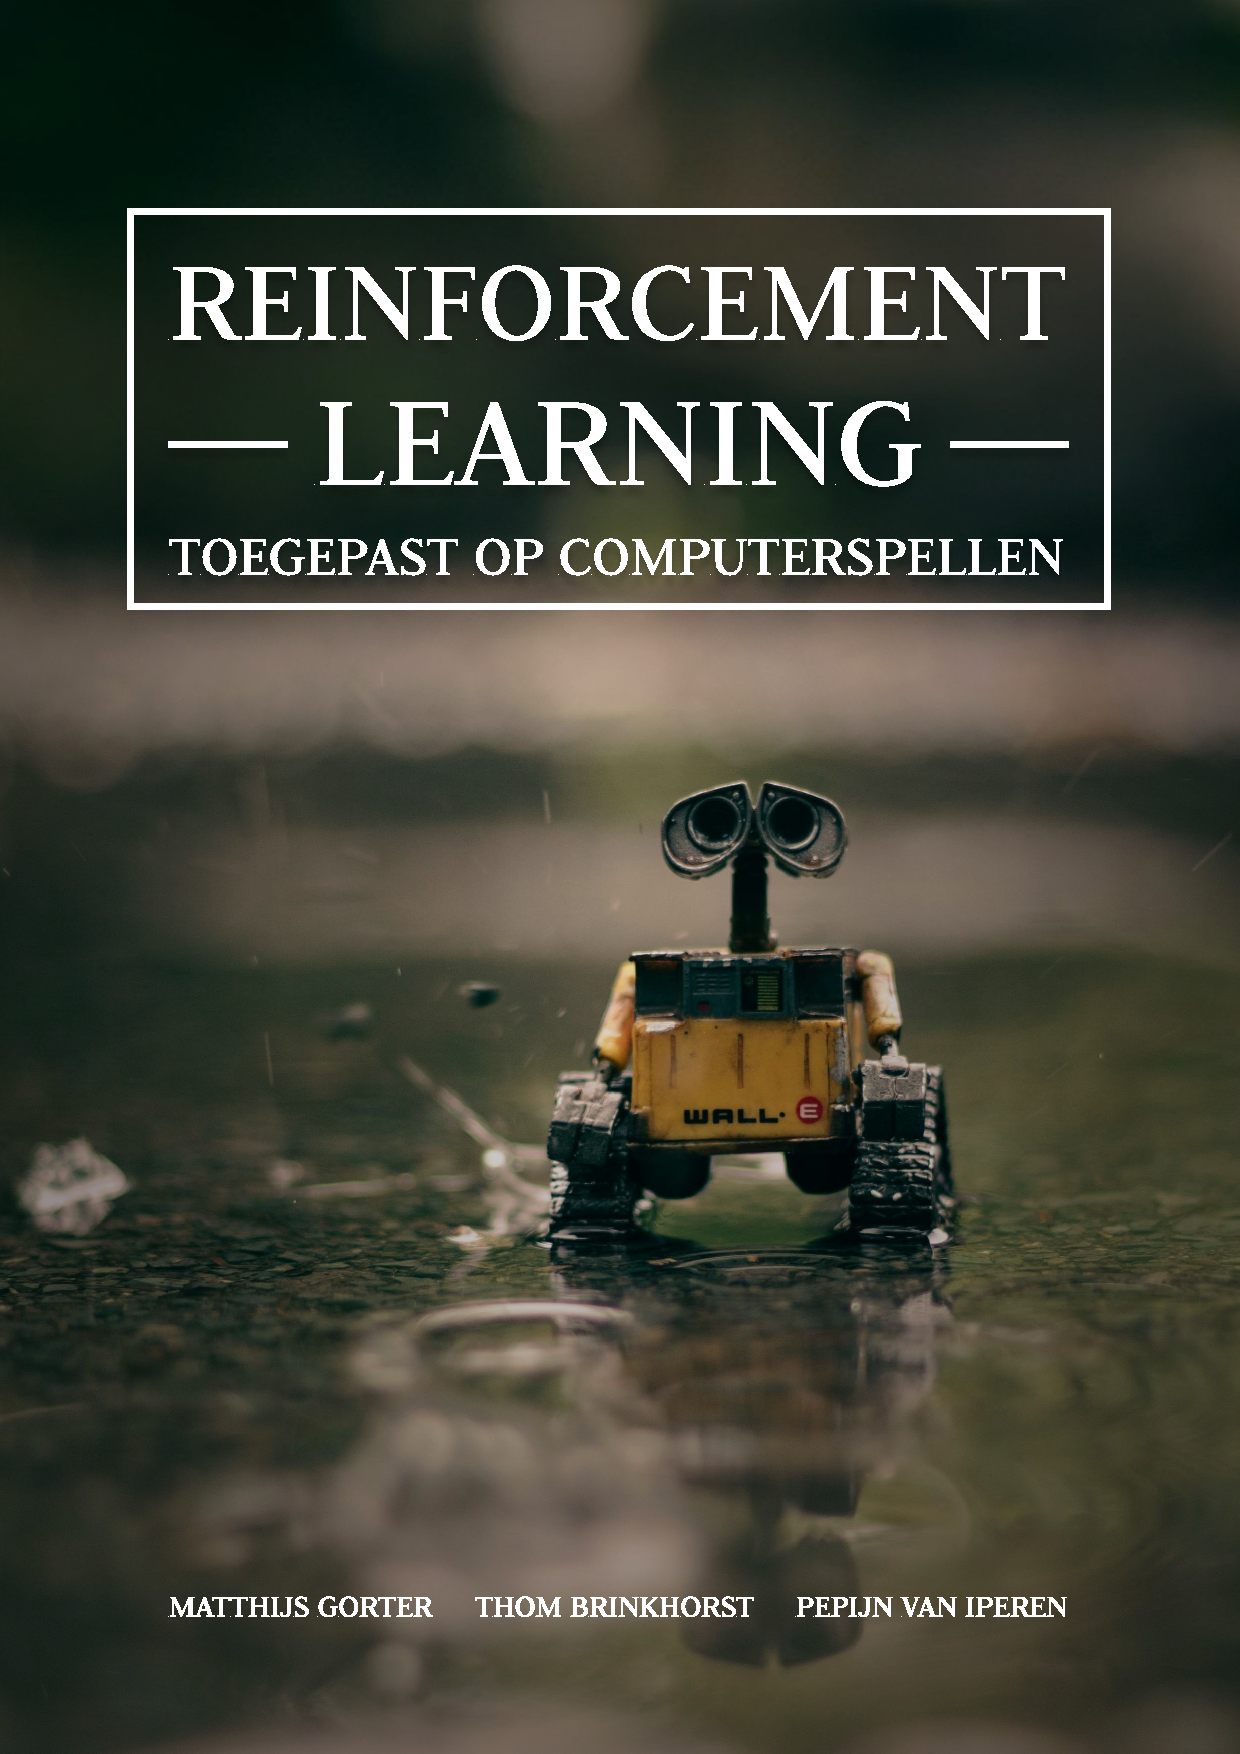
\includepdf[pages=1]{cover.pdf}

\begin{titlepage}
    \centering
    \vspace*{1cm}
    \Huge\textbf{Reinforcement Learning en Computerspellen} \\
    \vspace{1cm}
    \rule{\linewidth}{0.4mm}
    \Large
    Hoe beïnvloeden de specifieke kenmerken van computerspellen de effectiviteit van specifieke reinforcement learning-algoritmes?
    \rule{\linewidth}{0.4mm}

    \vspace{1.5cm}
    
\includegraphics[width=0.2\textwidth]{assets/logo-clz.png} \\
    \vspace{1.5cm}
    \large
    \textbf{Matthijs Gorter} \\
    \textbf{Thom Brinkhorst} \\
    \textbf{Pepijn van Iperen} \\
    \vspace{\fill}
    \normalsize

    Profielwerkstuk \\ onder begeleiding van \\ \textit{\textbf{S. Rook}} \\
    Christelijk Lyceum Zeist \\ Natuur en Techniek \\ Februari 2025 \\ \newpage
\end{titlepage}

\chapter*{Voorwoord}
\addcontentsline{toc}{chapter}{Voorwoord} % Voeg toe aan de inhoudsopgave

Toen we begonnen na te denken over een onderwerp voor ons profielwerkstuk,
wilden we graag een thema kiezen dat zowel uitdagend als actueel was.
Kunstmatige intelligentie (KI) houdt ons al enige tijd bezig, vooral vanwege de
invloed die het heeft op onze toekomst en de vele toepassingen die het nu al
kent. Het idee om ons te verdiepen in reinforcement learning ontstond omdat
deze tak van KI niet alleen theoretisch interessant is, maar ook praktisch
ontzettend krachtig is.

Reinforcement learning staat aan de basis van indrukwekkende prestaties, zoals
zelflerende spelprogramma’s, geavanceerde robotsystemen en zelfrijdende auto’s.
De manier waarop een computer ‘leert’ door beloningen en straffen sprak ons
aan, omdat het lijkt op hoe wij als mensen leren. Het leek ons daarom een
perfecte uitdaging om dit complexe onderwerp te onderzoeken en te begrijpen hoe
het precies werkt.

Matthijs Gorter, Thom Brinkhorst, Pepijn van Iperen \\ Christelijk Lyceum Zeist
\\ Februari 2025

\tableofcontents
\newpage
\pagenumbering{arabic}  % Overschakelen naar Arabische nummering
\chapter*{Notatie}
\addcontentsline{toc}{chapter}{Notatie} % Voeg toe aan de Inhoudsopgave
\begin{table}[h]
    \begin{tabular}{>{\raggedright}p{2.5cm} >{\raggedright\arraybackslash}p{10cm}}
        \textbf{Variabele}       & \textbf{Definitie}                          \\
        \rule{\linewidth}{0.4mm} & \rule{\linewidth}{0.4mm}                    \\
        $t$                      & Tijdstap                                    \\
        $T$                      & Laatste tijdstap van een episode            \\
        $x$                      & Toestand                                    \\
        $x_t$                    & Toestand op tijdstap $t$                    \\
        $x'$                     & De volgende toestand                        \\
        $\mathcal{X}$            & Toestandsruimte                             \\
        $a$                      & Actie                                       \\
        $\mathcal{A}$            & Actieruimte                                 \\
        $a_t$                    & Actie op tijdstip $t$                       \\
        $r$                      & Beloning                                    \\
        $\mathcal{R}$            & Beloningsruimte                             \\
        $r_t$                    & Beloning op tijdstip $t$                    \\
        $r(x, a)$                & Beloningsfunctie                            \\
        $\mu$                    & Deterministisch beleid                      \\
        $\pi$                    & Stochastisch beleid                         \\
        $\pi^*$                  & Optimale stochastisch beleid                \\
        $\alpha$                 & Leersnelheid tussen 0 en 1                  \\
        $\gamma$                 & Kortingsfactor tussen 0 en 1                \\
        $\epsilon$               & Exploratieparameter tussen 0 en 1           \\
        $p(x'|x, a)$             & Overgangswaarschijnlijkheidsfunctie         \\
        $V(x)$                   & Waardefunctie                               \\
        $Q(x, a)$                & Q-functie                                   \\
        $\mathbb{E}[X]$          & Verwachtingswaarde van variabele $X$        \\
        $\theta$                 & De gewichten van het hoofd neuraal netwerk  \\
        $\theta^-$               & De gewichten van het target netwerk         \\
        $\Phi$                   & De voorbewerkte toestand                    \\
        $\mathcal{D}$            & Replay-geheugen voor opslag van transities. \\
        $\mathcal{N}$            & Capaciteit van het replay-geheugen          \\
        $y_j$                    & Doelwaarde voor training                    \\

    \end{tabular}
    \caption{Notatie}
\end{table}

\newpage

\chapter{Inleiding}
Reinforcement Learning (RL) is een tak binnen de kunstmatige intelligentie die
zich richt op het trainen van een agent om optimale acties te ondernemen binnen
een specifieke omgeving. Een agent is een entiteit die leert en acties
onderneemt. Bij een zelfrijdende auto is het besturingssysteem de agent, en bij
een schaakspel is de schaker de agent.

\noindent
\begin{minipage}[t]{0.65\textwidth}
    \vspace{-6.5\baselineskip}
    De omgeving is alles waarmee de agent interacteert en die reageert op de acties van
    de agent. Bij een zelfrijdende auto is dit de weg waar de auto op rijdt en de
    voertuigen om de auto heen. Bij een schaakspel is dit het schaakbord. De agent
    leert door interactie met zijn omgeving. De agent ontvangt beloningen of
    straffen (negatieve beloningen) als gevolg van zijn acties. Het doel van de
    agent is om een strategie te ontwikkelen die de cumulatieve beloning
    maximaliseert over tijd.
\end{minipage}
\hfill % Ruimte tussen de twee minipages
\begin{minipage}[t]{0.3\textwidth} % Breedte aanpassen naar wens
    \centering
    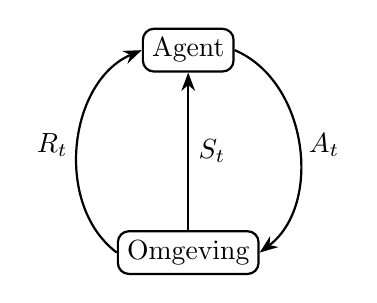
\begin{tikzpicture}[auto, thick, node distance=2cm, >=Stealth]
        % Nodes
        \node[draw, rectangle, rounded corners] (agent) {Agent};
        \node[draw, rectangle, rounded corners, below=of agent] (environment) {Omgeving};

        % Actie-pijl
        \draw[->] (agent.east) to[bend left=60] node[midway, right] {$A_t$} (environment.east);

        % Toestand-pijl
        \draw[->] (environment.north) to node[midway, right] {$S_{t}$} (agent.south);

        % Beloning-pijl
        \draw[->] (environment.west) to[bend left=60] node[midway, left] {$R_{t}$} (agent.west);
    \end{tikzpicture}
    \captionof{figure}{RL model tussen agent en omgeving.}
    \label{fig:rl_model}
\end{minipage}

Dit proces vindt plaats door middel van een vallen en opstaan aanpak, waarbij
de agent beloningen ontvangt voor correcte acties en straffen voor incorrecte
acties(negatieve beloningen). Het uiteindelijke doel is het maximaliseren van
de cumulatieve beloning over tijd.

Computerspellen vormen een ideaal testplatform voor RL vanwege de veelzijdige
uitdagingen die ze bieden, zoals dynamische omgevingen, complexe regels en
onvoorspelbare scenario’s. RL wordt gebruikt in veel verschillende spellen,
variërend van actiespellen zoals Snake tot strategische spellen zoals Schaken.

\section{Doel van het onderzoek}
Het doel van dit onderzoek is om te begrijpen hoe de kenmerken van
verschillende computerspellen de effectiviteit van verschillende reinforcement
learning (RL) algoritmes beïnvloeden bij het verbeteren van spelprestaties. Dit
onderzoek richt zich op het identificeren van de eigenschappen van
verschillende soorten spellen en de kenmerken van RL-algoritmes.

Door verschillende RL-algoritmes toe te passen op een reeks spellen met
verschillende kenmerken, willen we ontdekken welke algoritmes het beste
presteren in welke soorten spellen. Dit kan variëren van strategische spellen
die planning vereisen tot actiespellen die snelle beslissingen vragen.
\section{Onderzoeksvragen}
\subsection*{Hoofdvraag}
Hoe beïnvloeden de specifieke kenmerken van computerspellen de effectiviteit
van verschillende reinforcement learning-algoritmes in het optimaliseren van
spelprestaties?
\subsection*{Deelvragen}
Om beter te begrijpen hoe de kenmerken van computerspellen de prestaties van
verschillende reinforcement learning (RL) algoritmes beïnvloeden, hebben we
drie belangrijke deelvragen opgesteld
\begin{enumerate}

    \item\subsubsection*{Wat zijn de specifieke kenmerken van verschillende soorten computerspellen?}
          Deze vraag richt zich de eigenschappen van
          verschillende soorten computerspellen. Spellen kunnen sterk verschillen in
          hoe ze zijn opgebouwd, hoe snel spelers beslissingen moeten nemen en hoe
          complex de spelregels zijn. Door deze kenmerken te onderzoeken, kunnen
          we inzicht krijgen in welke aspecten van een spel een uitdaging vormen voor RL-algoritmes.

    \item\subsubsection*{Welke reinforcement learning-algoritmes zijn beschikbaar en wat zijn hun
              kenmerken?}
          Hier willen we kijken naar de verschillende soorten RL-algoritmes die beschikbaar
          zijn en wat hen uniek maakt. Sommige algoritmes zijn beter in het leren van eenvoudige
          taken, terwijl andere juist goed zijn in het omgaan met complexe situaties.

    \item\subsubsection*{Hoe beïnvloeden de spelkenmerken de prestatie van reinforcement learning-algoritmes?}

          Deze vraag gaat in op het belangrijkste deel van het onderzoek: het verband
          tussen de kenmerken van een spel en hoe goed een RL-algoritme presteert. We
          willen weten hoe bepaalde eigenschappen van een spel, zoals de noodzaak voor
          snelle beslissingen of lange-termijnplanning, invloed hebben op de
          effectiviteit van een algoritme. Door de prestaties van verschillende
          algoritmes in verschillende spellen te vergelijken, kunnen we ontdekken welke
          het beste werken voor bepaalde soorten spellen en waarom dat zo is.

\end{enumerate}
\section{Hypothese}
We verwachten dat:
\begin{enumerate}
    \item Deep Q-Network het beste zal presteren in Snake omdat het algoritme snel kan
          leren in omgevingen met beperkte ruimte en snel veranderende situaties, waar
          directe beloningen een grote rol spelen.

    \item Proximal Policy Optimization zal beter presteren in Mario Super Bros, omdat dit
          algoritme geschikt is voor dynamische omgevingen en situaties waar zowel
          snelheid en planning belangrijk zijn.

    \item AlphaZero zal beter zijn in Schaken, vanwege het planning en
          lange-termijnstrategie die nodig zijn.

\end{enumerate}

\section{Relevantie van het Onderzoek}
Dit onderzoek laat effectiviteit van reinforcement learning algoritmes in
verschillende omgevingen laat zien, wat bijdraagt aan het beter gebruik van
KI-systemen. Deze kennis kan niet alleen worden toegepast binnen de
game-industrie, maar ook in andere sectoren zoals de gezondheidszorg,
zelfrijdende auto's en robotica.

\chapter{Theoretisch Kader}

Reinforcement Learning (RL) opereert binnen het kader van Markov Decision
Processes (MDP's), die een wiskundige basis bieden voor het modelleren van
sequentiële beslissingsproblemen. Dit hoofdstuk bespreekt belangrijke de
concepten in RL.

\section{Fundamentele Elementen van MDP's}

\subsection{Toestandsruimte}
Laat (\(\mathcal{X}\)) de toestandsruimte zijn, waarbij elke toestand (\(x \in
\mathcal{X}\)) de huidige situatie of staat is van de omgeving waarin de agent
opereert. Op de aanvangsstap (\(t = 0\)) begint de agent in een initiële
toestand (\(x_0\)). Naarmate het proces vordert, bevindt de agent zich in
nieuwe toestanden gebaseerd op zijn acties.

\subsection{Actieruimte}
Laat (\(\mathcal{A}\)) de actieruimte zijn, waarbij elke actie (\(a \in
\mathcal{A}\)) een mogelijke beslissing van de agent vertegenwoordigt. De
interactie tussen de agent en de omgeving verloopt in discrete tijdstappen (\(t
= 0, 1, 2, \ldots, T\)), waarbij de horizon (\(T\)) eindig of oneindig kan
zijn.

\subsection{Beloningsfunctie}
De beloningsfunctie (\(r: \mathcal{X} \times \mathcal{A} \to \mathbb{R}\))
koppelt toestand-actieparen aan beloningen, waarbij (\(r(x,a)\)) de directe
beloning vertegenwoordigt die wordt ontvangen na het uitvoeren van actie
(\(a\)) in toestand (\(x\)).

\section{Markov-eigenschap en Overgangsdynamiek}

\subsection{De Markov-eigenschap}
Het onderscheidende kenmerk van MDP's is de Markov-eigenschap, die stelt dat de
toekomstige toestand alleen afhankelijk is van de huidige toestand en actie,
onafhankelijk van de geschiedenis:
\begin{equation}
    p(x_{t+1}|x_t,a_t,x_{t-1},a_{t-1},\ldots,x_0,a_0) = p(x_{t+1}|x_t,a_t)
\end{equation}
Voorbeeld van het Markov-eigenschap:
\begin{itemize}
    \item \textbf{Snake}: De toekomstige toestand (positie van de slang en voedsel) is volledig bepaald door de huidige toestand (huidige positie en locatie van het voedsel) en de actie (richting van beweging) zonder afhankelijk te zijn van de geschiedenis van eerdere bewegingen.
\end{itemize}

Voorbeeld van geen Markov-eigenschap:
\begin{itemize}
    \item \textbf{Poker}: De beslissingen in poker zijn afhankelijk van niet alleen de huidige hand, maar ook van de geschiedenis van inzetten en het gedrag van andere spelers in vorige rondes.
\end{itemize}

\subsection{Overgangswaarschijnlijkheidsfunctie}
Voor eindige toestands- en actieruimten (\(|\mathcal{X}|, |\mathcal{A}| <
\infty\)) worden de overgangsdynamieken beschreven door een
waarschijnlijkheidsfunctie (\(p: \mathcal{X} \times \mathcal{A} \times
\mathcal{X} \to [0,1]\)), waarbij (\(p(x'|x,a)\)) de waarschijnlijkheid
vertegenwoordigt om over te gaan naar toestand (\(x'\)) gegeven de huidige
toestand (\(x\)) en actie (\(a\)).

\section{Beleid en Verwachte Waarden}

\subsection{Beleid}
In RL is een beleid de strategie die een agent volgt om beslissingen te nemen.
Het bepaalt welke actie een agent moet uitvoeren, gegeven de huidige toestand
van de omgeving. Een beleid in reinforcement learning kan op twee manieren
worden gedefinieerd:

\begin{itemize}
    \item \textbf{Deterministisch Beleid:} \\
          \(\pi: \mathcal{X} \to \mathcal{A}\), waarbij \(a_t = \pi(x_t)\) \\
          Voor elke toestand \(x_t\) schrijft het beleid exact één actie \(a_t\) voor.

    \item \textbf{Stochastisch Beleid:} \\
          \(\pi: \mathcal{X} \times \mathcal{A} \to [0,1]\), waarbij \(\pi(a|x)\) de waarschijnlijkheid geeft van het kiezen van actie \(a\) in toestand \(x\) \\
          Voor een gegeven toestand \(x\) definieert het beleid een waarschijnlijkheidsverdeling over mogelijke acties.
\end{itemize}

\subsection{Verwachte Waarden}
De verwachtingswaarde \(\mathbb{E}[X]\) (Expected value), of het gemiddelde,
van een willekeurige variabele \(X\) is een manier om het gemiddelde resultaat
te berekenen dat je zou verwachten als je een groot aantal experimenten
uitvoert. Bijvoorbeeld, als \(X\) een dobbelsteenworp vertegenwoordigt, dan is
\(\mathbb{E}[X]\) het gemiddelde van de uitkomsten 1, 2, 3, 4, 5, en 6, wat
gelijk is aan 3,5. De conditionele verwachting (\(\mathbb{E}[X|Y]\)) geeft de
verwachte waarde van (\(X\)) gegeven (\(Y\)).

\section{Leerparameters in Reinforcement Learning}

Bij reinforcement learning spelen verschillende hyperparameters een cruciale
rol in het leerproces van de agent. Drie van de belangrijkste parameters zijn
het leerpercentage (\(\alpha\)), de kortingsfactor (\(\gamma\)), en de
exploratieparameter (\(\epsilon\)). Deze worden hieronder uitgelegd.

\subsection{Leerpercentage}

Het leerpercentage (\(\alpha\)) bepaalt hoe sterk nieuwe informatie wordt
gewogen ten opzichte van bestaande kennis.

De waarde van \(\alpha\) ligt tussen \(0\) en \(1\):
\begin{itemize}
    \item Als \(\alpha = 0\): De agent leert niets; bestaande kennis blijft onveranderd.
    \item Als \(\alpha = 1\): Alleen nieuwe informatie wordt gebruikt; bestaande kennis
          wordt genegeerd.
    \item Voor \(0 < \alpha < 1\): Oude en nieuwe informatie worden gecombineerd, wat
          doorgaans de voorkeur heeft.
\end{itemize}

\subsection{Kortingsfactor}

De kortingsfactor (\(\gamma\)) bepaalt hoe belangrijk toekomstige beloningen
zijn in vergelijking met onmiddellijke beloningen. Het beïnvloedt de totale
beloning die de agent probeert te maximaliseren. De totale beloning wordt
gedefinieerd als:

\begin{equation}
    R = \sum_{t=0}^\infty \gamma^t r_t
\end{equation}

Waarbij \(r_t\) de beloning is die ontvangen wordt op tijdstip \(t\). De waarde
van \(\gamma\) varieert meestal tussen \(0\) en \(1\):
\begin{itemize}
    \item Als \(\gamma = 0\): Alleen directe beloningen worden overwogen.
    \item Als \(\gamma = 1\): Toekomstige beloningen zijn even belangrijk als directe
          beloningen.
    \item Voor \(0 < \gamma < 1\): Toekomstige beloningen worden gedisconteerd, met een
          lagere waarde naarmate ze verder in de toekomst liggen.
\end{itemize}

\subsection{Exploratieparameter}

De exploratieparameter (\(\epsilon\)) wordt gebruikt in de epsilon-greedy
strategie om een balans te vinden tussen exploratie (het verkennen van nieuwe
acties) en exploitatie (het uitvoeren van de momenteel beste actie). De
strategie werkt als volgt. Met kans \(\epsilon\): Kies een willekeurige actie
(exploratie). Anders kiest de agent de actie die momenteel de hoogste geschatte
Q-waarde heeft (exploitatie).

De waarde van \(\epsilon\) bepaalt het gedrag van de agent:
\begin{itemize}
    \item Als \(\epsilon = 0\): De agent exploiteert alleen, wat kan leiden tot
          suboptimale oplossingen.
    \item Als \(\epsilon = 1\): De agent verkent alleen, zonder gericht gebruik van
          kennis.
\end{itemize}

\section{Waarde-functies}
De toestandswaarde-functie geeft aan hoe goed een bepaalde toestand is, terwijl
de Q-functie aangeeft hoe goed een actie in een bepaalde toestand is.
\subsection{Toestandswaarde-functie}
De toestandswaarde-functie (\(V^\pi: \mathcal{X} \to \mathbb{R}\)) onder beleid
(\(\pi\)) wordt gedefinieerd als:
\begin{equation}
    V^\pi(x) = \mathbb{E}_\pi\left[\sum_{t=0}^\infty \gamma^t r_t \mid x_0 = x\right]
\end{equation}
Deze functie geeft de verwachte waarde van de totale beloning die een agent zal
ontvangen vanaf de toestand \(x\).
\subsection{Q-functie}
De Q-functie (\(Q^\pi: \mathcal{X} \times \mathcal{A} \to \mathbb{R}\)) onder
beleid (\(\pi\)) wordt gedefinieerd als:
\begin{equation}
    Q^\pi(x,a) = \mathbb{E}_\pi\left[\sum_{t=0}^\infty \gamma^t r_t \mid x_0 = x, a_0 = a\right]
\end{equation}
Deze functie geeft de verwachte waarde van de totale beloning die een agent zal
ontvangen vanaf de toestand \(x\) en na het nemen van actie \(a\).

\chapter{Kenmerken van specifieke Algoritmes}

\section{Q-Learning}
Q-learning, geïntroduceerd door Chris Watkins in 1989, is een van de
belangrijkste vooruitgangen binnen reinforcement learning. Dit model-vrije,
off-policy algoritme is een van de meest gebruikte algoritmen binnen
reinforcement learning vanwege zijn eenvoud en effectiviteit.
\subsection{Proces}
Het proces van het Q-learning-algoritme, zoals weergegeven in
\textbf{Algoritme~\ref{alg:Q-learning}} en de flowchart in
\textbf{Figuur~\ref{fig:ql_flowchart}}, begint met het opstellen van een
Q-tabel. Deze tabel bevat de Q-waarden voor alle combinaties van toestanden en
acties. Aan het begin zijn alle waarden ingesteld op nul.

Vervolgens start het spel, waarbij de agent de volgende actie bepaalt. Hierbij
heeft de agent twee mogelijkheden:
\begin{itemize}
    \item Exploratie: De agent voert een willekeurige actie uit om nieuwe informatie te
          verkennen.
    \item Exploitatie: De agent selecteert een actie op basis van de bestaande Q-tabel,
          waarbij de actie met de hoogste Q-waarde in de huidige toestand wordt gekozen.
\end{itemize}

De keuze tussen exploratie en exploitatie wordt bepaald door de parameter
$\epsilon$. De kans dat de agent een willekeurige actie uitvoert (exploratie)
is gelijk aan $\epsilon$. Aan het begin van de training is $\epsilon$ gelijk
aan 1, en deze waarde neemt exponentieel af naarmate de training vordert. Tegen
het einde van de training is $\epsilon$ vrijwel 0.

Nadat een actie is uitgevoerd, ontvangt de agent een beloning. Op basis van
deze beloning wordt de Q-waarde voor de combinatie van de uitgevoerde actie en
de huidige toestand bijgewerkt in de Q-tabel zoals te zien is in formule
\eqref{eq:Q-functie}. Dit proces wordt herhaald totdat de training is voltooid.

\begin{algorithm}
    \caption{Q-Learning Algoritme}\label{alg:Q-learning}
    \begin{algorithmic}
        \State \textbf{Initialisatie:} Stel $Q(s, a)$ willekeurig in voor alle toestanden $s$ en acties $a$
        \For{elke episode}
        \State Initialiseer begin-toestand $s$
        \While{$s$ is niet een terminale toestand}
        \State Kies actie $a$ in toestand $s$ op basis van een beleid $\pi$
        \State Voer actie $a$ uit, observeer beloning $r$ en de volgende toestand $s'$
        \State Update de Q-waarde:
        \begin{equation} \label{eq:Q-functie}
            Q(x, a) \leftarrow Q(x, a) + \alpha \left[ r + \gamma \max_{a'} Q(x', a') - Q(x, a) \right]
        \end{equation}

        \State $s \gets s'$
        \EndWhile
        \EndFor
    \end{algorithmic}
\end{algorithm}

\begin{figure}
    \centering
    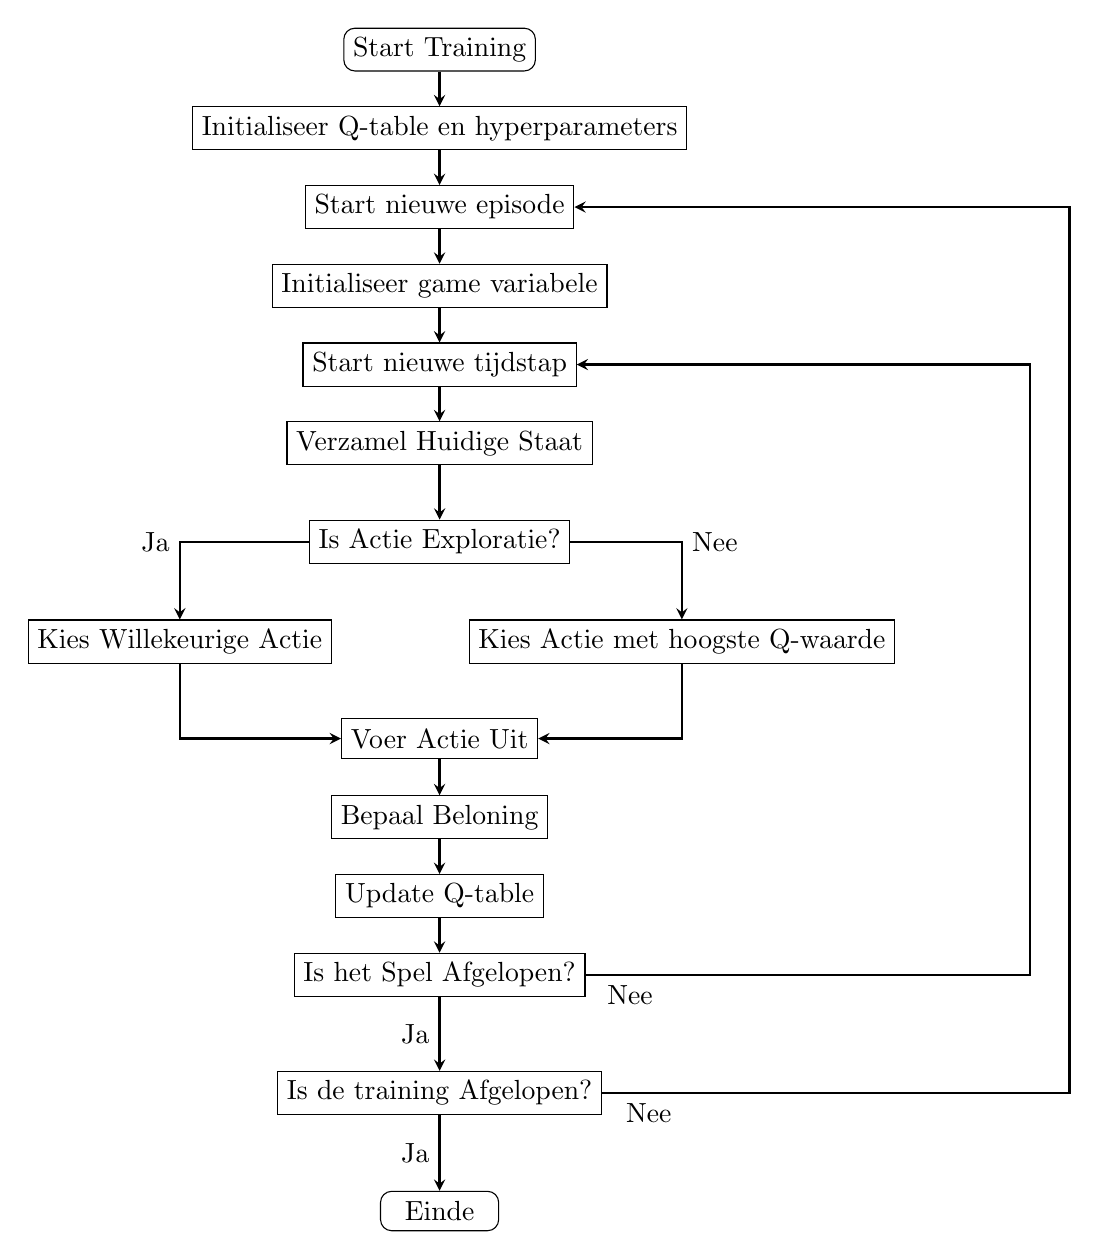
\begin{tikzpicture}[node distance=1cm, auto, >=latex']
        % Definieer stijlen voor verschillende soorten knooppunten
        \tikzstyle{startstop} = [rectangle, rounded corners, minimum width=1.5cm, minimum height=0.5cm,text centered, draw=black, fill=red!0]
        \tikzstyle{process} = [rectangle, minimum width=1.5cm, minimum height=0.5cm, text centered, draw=black, fill=orange!0]
        \tikzstyle{decision} = [rectangle, minimum width=1.5cm, minimum height=0.5cm, text centered, draw=black, fill=green!0]
        \tikzstyle{arrow} = [thick,->,>=stealth]

        % Knopen plaatsen
        \node (start) [startstop] {Start Training};
        \node (trainingInit) [process, below of=start] {Initialiseer Q-table en hyperparameters};
        \node (startEpisode) [process, below of=trainingInit] {Start nieuwe episode};
        \node (episodeInit) [process, below of=startEpisode] {Initialiseer game variabele};
        \node (startTimestep) [process, below of=episodeInit] {Start nieuwe tijdstap};
        \node (getstate) [process, below of=startTimestep] {Verzamel Huidige Staat};
        \node (decideexplore) [decision, below of=getstate, yshift=-0.25cm] {Is Actie Exploratie?};
        \node (explore) [process, below left=of decideexplore, xshift=1cm] {Kies Willekeurige Actie};
        \node (exploit) [process, below right=of decideexplore, xshift=-2cm] {Kies Actie met hoogste Q-waarde};
        \node (executeaction) [process, below of=decideexplore, yshift=-1.5cm] {Voer Actie Uit};
        \node (determinereward) [process, below of=executeaction] {Bepaal Beloning};
        \node (updateq) [process, below of=determinereward] {Update Q-table};
        \node (checkgameover) [decision, below of=updateq] {Is het Spel Afgelopen?};
        \node (checktrainingover) [decision, below of=checkgameover, yshift=-0.5cm] {Is de training Afgelopen?};
        \node (stop) [startstop, below of=checktrainingover, yshift=-0.5cm] {Einde};

        % Pijlen tekenen
        \draw [arrow] (start) -- (trainingInit);
        \draw [arrow] (trainingInit) -- (startEpisode);
        \draw [arrow] (startEpisode) -- (episodeInit);
        \draw [arrow] (episodeInit) -- (startTimestep);
        \draw [arrow] (startTimestep) -- (getstate);
        \draw [arrow] (getstate) -- (decideexplore);
        \draw [arrow] (decideexplore) -| node[anchor=east] {Ja} (explore);
        \draw [arrow] (decideexplore) -| node[anchor=west] {Nee} (exploit);
        \draw [arrow] (explore) |- (executeaction);
        \draw [arrow] (exploit) |- (executeaction);
        \draw [arrow] (executeaction) -- (determinereward);
        \draw [arrow] (determinereward) -- (updateq);
        \draw [arrow] (updateq) -- (checkgameover);
        \draw [arrow] (checkgameover) -- node[anchor=east] {Ja} (checktrainingover);
        \draw [arrow] (checkgameover) -| node[pos=0.05, anchor=north, align=center] {Nee} (7.5,-4) -- (startTimestep);
        \draw [arrow] (checktrainingover) -- node[anchor=east] {Ja} (stop);
        \draw [arrow] (checktrainingover) -| node[pos=0.05, anchor=north, align=center] {Nee} (8,-2) -- (startEpisode);
    \end{tikzpicture}
    \caption{Flowchart van het Q-Learning Algoritme}\label{fig:ql_flowchart}
\end{figure}

\subsection{Beperkingen}
Een van de grootste beperkingen van Q-learning is schaalbaarheid. De
toestandsruimte neemt exponentieel toe wanneer het aantal dimensies toeneemt:
\begin{equation}
    |\mathcal{S}| = d^n
\end{equation}
waarbij $d$ het aantal mogelijke waarden per dimensie is en $n$ het aantal
dimensies.

Dit leidt tot hoge eisen aan geheugen en rekenkracht:
\begin{equation}
    \text{Complexiteit} = O(|\mathcal{S}| \times |\mathcal{A}|)
\end{equation}
\section{Deep Q-Network}
Deep Q-Network (DQN), geïntroduceerd door DeepMind in 2013 combineert
Q-learning met diepe neurale netwerken. Deze innovatie maakte het mogelijk om
reinforcement learning toe te passen op problemen met grootte toestandruimtes,
zoals pixels van videospellen.

\subsection{Neuraal Netwerk}
Het DQN maakt gebruikt van neurale-netwerkarchitectuur die is ontworpen om de
optimale actie-waarde functie te benaderen. De netwerkarchitectuur,
geïllustreerd in Figuur \ref{fig:neuraal-netwerk}, is een typisch neuraal
netwerk in DQN.

\begin{figure}[h]

    \centering
    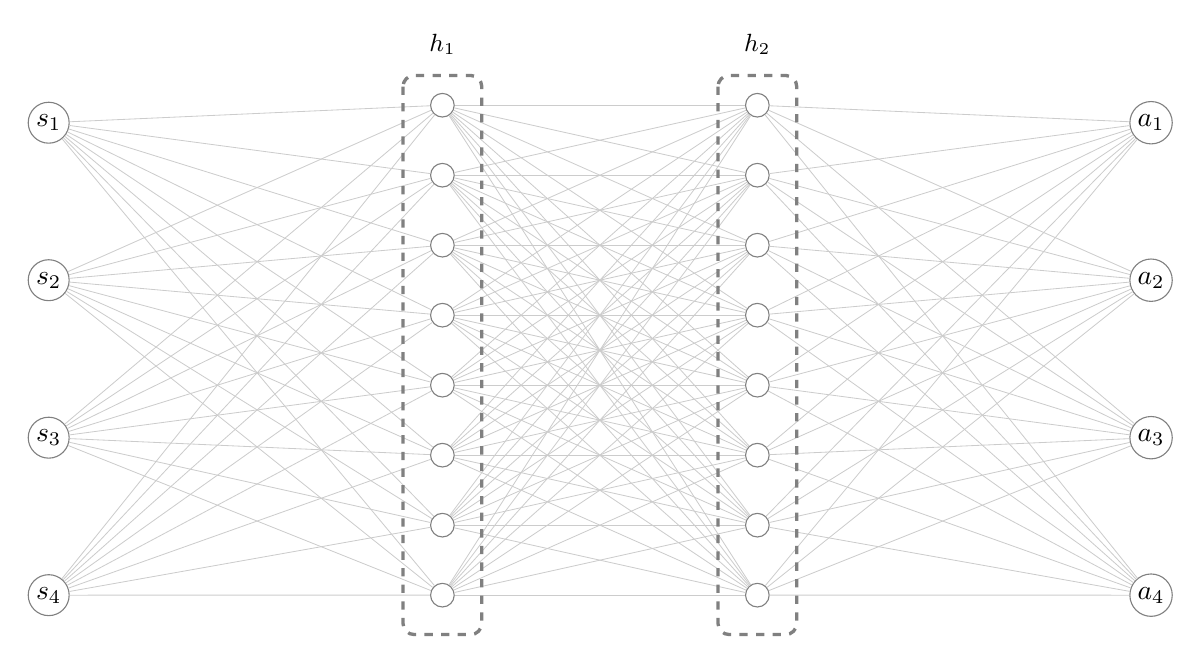
\begin{tikzpicture}[
            scale=2,
            node distance=5cm,
            every node/.style={
                    draw=black!30,
                    fill=white,
                    rounded corners=0.1cm,
                    minimum size=0.4cm,
                    inner sep=0.05cm,
                    text centered
                },
            input neuron/.style={
                    draw=black!50,
                    circle,
                    minimum size=0.3cm
                },
            hidden neuron/.style={
                    draw=black!50,
                    circle,
                    minimum size=0.3cm
                },
            output neuron/.style={
                    draw=black!50,
                    circle,
                    minimum size=0.3cm
                },
            connecting line/.style={
                    draw=black!20,
                    line width=0.3pt
                },
            layer label/.style={
                    text centered,
                    draw=black!0,
                    font=\small\sffamily
                },
            layer rectangle/.style={
                    draw=black!50,
                    rounded corners,
                    dashed,
                    very thick
                }
        ]

        % Input Layer
        \foreach \i [count=\y] in {1,...,4} {
                \node[input neuron] (input-\i) at (0, {-\y}) {$s_{\i}$};
            }

        % Hidden Layers
        \foreach \j in {1,...,2} {
                \foreach \i [count=\y] in {1,...,8} {
                        \node[hidden neuron] (hidden\j-\i) at ({0.5 + 2 * \j}, {-4/9-\y*4/9}) {};
                    }
            }

        % Output Layer
        \foreach \i [count=\y] in {1,...,4} {
                \node[output neuron] (output-\i) at (7, {-\y}) {$a_{\i}$};
            }

        % Connections
        \foreach \i in {1,...,4} {
                \foreach \j in {1,...,8} {
                        \draw[connecting line] (input-\i) -- (hidden1-\j);
                    }
            }

        \foreach \i in {1,...,8} {
                \foreach \j in {1,...,8} {
                        \draw[connecting line] (hidden1-\i) -- (hidden2-\j);
                    }
            }

        \foreach \i in {1,...,8} {
                \foreach \j in {1,...,4} {
                        \draw[connecting line] (hidden2-\i) -- (output-\j);
                    }
            }

        % Layer labels
        \node[layer label] at (2.5, -0.50) {$h_1$};
        \node[layer label] at (4.5, -0.50) {$h_2$};

        % Layer rectangles
        \draw[layer rectangle] (2.25, -0.70) rectangle (2.75, -4.25);
        \draw[layer rectangle] (4.25, -0.70) rectangle (4.75, -4.25);

    \end{tikzpicture}
    \caption{Diagram van een typisch neuraal netwerk in een DQN met een invoerlaag, twee verborgen lagen en een uitvoerlaag.}
    \label{fig:neuraal-netwerk}
\end{figure}
Het neurale netwerk wordt gekenmerkt door de volgende architecturale elementen:

De \textbf{invoerlaag} bestaat uit een verzameling toestanden ${s_1, s_2,
            \ldots, s_n}$, waarbij elke toestand een neuron is en een specifieke
toestandseigenschap vastlegt. De \textbf{uitvoerlaag} bestaat verzameling
acties ${a_1, a_2, \ldots, a_n}$, waarbij elke actie. De \textbf{verborgen
    lagen} in een neuraal netwerk, genoteerd als \( h_1, h_2, \ldots, h_n \), zijn
de lagen die zich bevinden tussen de invoerlaag en de uitvoerlaag. Deze
verborgen lagen zijn belangrijk voor het leren en modelleren van complexe
patronen in de data. Elk neuron in een verborgen laag voert een bewerking uit
volgens de formule:

\begin{equation}
    h_j = f\left(\sum_{i} w_{ij} x_i + b_j\right),
\end{equation}

waarbij:
\begin{itemize}
    \item \( h_j \) de output van neuron \( j \) is,
    \item \( x_i \) de invoerwaarden zijn,
    \item \( w_{ij} \) de gewichten die de sterkte van de verbindingen tussen de invoer \( i \) en het neuron \( j \) vertegenwoordigen,
    \item \( b_j \) de bias-term,
    \item \( f(\cdot) \) de activatiefunctie.
\end{itemize}

In dit geval wordt de Rectified Linear Unit (ReLU) activatiefunctie gebruikt,
gedefinieerd als:

\begin{equation}
    f(x) = \max(0, x).
\end{equation}

De ReLU introduceert niet-lineariteit door negatieve waarden naar nul te
transformeren, terwijl positieve waarden onveranderd blijven. Deze
niet-lineariteit stelt het netwerk in staat om complexe functies te benaderen
die niet mogelijk zouden zijn met een louter lineaire transformatiestap.

Door de toepassing van \( n \) verborgen lagen, wordt een complexe
niet-lineaire transformatie uitgevoerd van de oorspronkelijke invoer \(
\mathbf{x} \) naar de uiteindelijke uitvoer \( \mathbf{y} \), als volgt:

\begin{equation}
    \mathbf{y} = f_n\left(W_n f_{n-1}\left(W_{n-1} \cdots f_1\left(W_1 \mathbf{x} + \mathbf{b}_1\right) \cdots + \mathbf{b}_{n-1}\right) + \mathbf{b}_n\right),
\end{equation}

waarbij \( W_i \) de gewichtsmatrix van laag \( i \) en \( \mathbf{b}_i \) de
bias-term van laag \( i \) vertegenwoordigen. Het gebruik van meerdere
verborgen lagen met ReLU maakt het netwerk krachtig genoeg om complexe patronen
te leren en invoeromstandigheden nauwkeurig te vertalen naar acties of
beslissingen.

\subsection{Proces}
Het Q-learning-algoritme, zoals weergegeven in \textbf{Algoritme~\ref{alg:DQN}}
en de flowchart in \textbf{Figuur~\ref{fig:dqn_flowchart}} breidt het
traditionele Q-learning uit door de Q-tabel te vervangen door een neuraal
netwerk. Dit netwerk leert de mapping tussen toestanden en Q-waarden voor alle
mogelijke acties. Het proces bestaat uit verschillende componenten die voor de
stabiliteit en effectiviteit van het algoritme zorgen. DQN maakt gebruik van
experience replay, waarbij ervaringen (toestand, actie, beloning, volgende
toestand) worden opgeslagen in een replay buffer en willekeurig worden gebruikt
voor training.

Daarnaast wordt een tweede neuraal netwerk, het target network, ingezet om de
doelwaarden te berekenen. Dit netwerk wordt regelmatig geüpdatet met de
gewichten van het hoofdnetwerk, wat de training verder stabiliseert. Voor
visuele inputs implementeert DQN convolutionele lagen die relevante informatie
halen uit de pixels, dit maakt het algorithme goed in het verwerken van
complexe visuele informatie.

\begin{algorithm}
    \caption{Deep Q-learning met Experience Replay \cite{dqn_paper}}\label{alg:DQN}
    \begin{algorithmic}
        \State Initialiseer replay-geheugen $\mathcal{D}$ met capaciteit $N$
        \State Initialiseer de actie-waarde functie $Q$ met willekeurige gewichten
        \For{elke episode $1, \dots, M$}
        \State Initialiseer sequentie $s_1 = \{x_1\}$ en preprocess $ \phi_1 = \phi(s_1)$
        \For{$t = 1, \dots, T$}
        \State Met kans $\epsilon$: kies een willekeurige actie $a_t$
        \State Anders: kies $a_t = \arg\max_a Q^*(\phi(s_t), a; \theta)$
        \State Voer actie $a_t$ uit in de omgeving en observeer beloning $r_t$ en beeld $x_{t+1}$
        \State Stel $s_{t+1} = s_t, a_t, x_{t+1}$ en preprocess $\phi_{t+1} = \phi(s_{t+1})$
        \State Sla transitie $(\phi_t, a_t, r_t, \phi_{t+1})$ op in $\mathcal{D}$
        \State Neem een willekeurige minibatch van transities $(\phi_j, a_j, r_j, \phi_{j+1})$ uit $\mathcal{D}$
        \State Bereken:
        \[
            y_j =
            \begin{cases}
                r_j                                              & \text{als } \phi_{j+1} \text{ terminaal is}      \\
                r_j + \gamma \max_{a'} Q(\phi_{j+1}, a'; \theta) & \text{als } \phi_{j+1} \text{ niet terminaal is}
            \end{cases}
        \]
        \State Voer een gradient-descent stap uit op $\left( y_j - Q(\phi_j, a_j; \theta) \right)^2$
        \EndFor
        \EndFor
    \end{algorithmic}
\end{algorithm}
\begin{figure}
    \centering
    \begin{tikzpicture}[node distance=0.8cm, auto, >=latex']
        % Definieer stijlen voor verschillende soorten knooppunten
        \tikzstyle{startstop} = [rectangle, rounded corners, minimum width=1.5cm, minimum height=0.5cm,text centered, draw=black, fill=red!0]
        \tikzstyle{process} = [rectangle, minimum width=1.5cm, minimum height=0.5cm, text centered, draw=black, fill=orange!0]
        \tikzstyle{decision} = [rectangle, minimum width=1.5cm, minimum height=0.5cm, text centered, draw=black, fill=green!0]
        \tikzstyle{arrow} = [thick,->,>=stealth]

        % Knopen plaatsen
        \node (start) [startstop] {Start Training};
        \node (init) [process, below of=start, yshift=-0.4cm] {Initialiseer replay-geheugen $\mathcal{D}$ en Q-functie};
        \node (episode) [process, below of=init, yshift=-0.4cm] {Start nieuwe episode};
        \node (initseq) [process, below of=episode, yshift=-0.4cm] {Initialiseer sequentie $s_1$ en $\phi_1$};
        \node (timestep) [process, below of=initseq, yshift=-0.4cm] {Start nieuwe tijdstap};

        \node (epsilon) [decision, below of=timestep, yshift=-0.4cm] {Is Actie Exploratie?};
        \node (random) [process, below left=of decideexplore, xshift=1cm] {Kies Willekeurige Actie};
        \node (maxq) [process, below right=of decideexplore, xshift=-2cm] {Kies Actie met hoogste Q-waarde};

        \node (execute) [process, below=2.5cm of epsilon] {Voer actie uit, observeer $r_t$ en $x_{t+1}$};
        \node (preprocess) [process, below of=execute, yshift=-0.4cm] {Update $s_{t+1}$ en bereken $\phi_{t+1}$};
        \node (store) [process, below of=preprocess, yshift=-0.4cm] {Sla transitie op in $\mathcal{D}$};
        \node (sample) [process, below of=store, yshift=-0.4cm] {Sample minibatch uit $\mathcal{D}$};
        \node (update) [process, below of=sample, yshift=-0.4cm] {Update Q-functie met gradient descent};

        \node (episodeend) [decision, below of=update, yshift=-1cm] {Episode afgelopen?};
        \node (trainingend) [decision, below of=episodeend, yshift=-1cm] {Training afgelopen?};
        \node (stop) [startstop, below of=trainingend, yshift=-0.4cm] {Einde Training};

        % Pijlen tekenen
        \draw [arrow] (start) -- (init);
        \draw [arrow] (init) -- (episode);
        \draw [arrow] (episode) -- (initseq);
        \draw [arrow] (initseq) -- (timestep);
        \draw [arrow] (timestep) -- (epsilon);
        \draw [arrow] (epsilon) -| node[left] {Ja} (random);
        \draw [arrow] (epsilon) -| node[right] {Nee} (maxq);
        \draw [arrow] (random) |- (execute);
        \draw [arrow] (maxq) |- (execute);
        \draw [arrow] (execute) -- (preprocess);
        \draw [arrow] (preprocess) -- (store);
        \draw [arrow] (store) -- (sample);
        \draw [arrow] (sample) -- (update);
        \draw [arrow] (update) -- (episodeend);
        \draw [arrow] (episodeend) -- node[right] {Ja} (trainingend);
        \draw [arrow] (episodeend) -| node[near start, above] {Nee} ++(7,0) |- (timestep);
        \draw [arrow] (trainingend) -- node[right] {Ja} (stop);
        \draw [arrow] (trainingend) -| node[near start, above] {Nee} ++(8,0) |- (episode);
    \end{tikzpicture}
    \caption{Flowchart van het Deep Q-learning met Experience Replay Algoritme}
    \label{fig:dqn_flowchart}
\end{figure}

\subsection{Verbeteringen op Klassiek Q-learning}
DQN lost verschillende problemen van Q-learning op. Het neurale netwerken zorgt
dat het algoritme in staat om effectief om te gaan met continue en
hoog-dimensionale toestandsruimtes. Het netwerk bezit ook sterke
generalisatie-eigenschappen, waardoor het patronen kan herkennen en toepassen
op ongeziene toestanden. De stabiliteit van het leerproces wordt significant
verbeterd door de introductie van experience replay en target networks, wat een
belangrijke vooruitgang is ten opzichte van Q-learning methoden.

\subsection{Voordelen en Beperkingen}
DQN is goed in complexe taken met visuele inputs effectief aan pakken zonder je
dat handmatige features moet selecteren. Het algoritme heeft goede
generalisatie-eigenschappen, waardoor het zich kan aanpassen aan nieuwe
situaties binnen het geleerde domein. Deze voordelen worden echter vergezeld
door beperkingen. DQN is computationeel intensief, het vereist grote
hoeveelheden trainingsdata om tot goede resultaten te komen. Daarnaast is het
algoritme gevoelig voor de keuze van hyperparameters, wat het
optimalisatieproces complex maakt.

\subsection{Toepassingen}
DQN wordt gebruikt in veel toepassingsgebieden. Bij van videogames heeft het
algoritme indrukwekkende resultaten behaald, met name bij het leren spelen van
Atari 2600 spellen op menselijk en bovenmenselijk niveau. Bij robotica en
motion control biedt DQN nieuwe mogelijkheden voor het ontwikkelen van
verfijnde besturingsstrategieën. Ook binnen autonome systemen wordt DQN
gebruikt door complexe beslissingsprocessen te optimaliseren.

\section{Deep   Policy Gradient}
Deep Deterministic Policy Gradient (DDPG), ontwikkeld door onderzoekers van
DeepMind in 2015, is een algoritme dat zich richt op continue actieruimtes. Als
een uitbreiding op de policy gradient methoden en Actor-Critic architecturen,
combineert DDPG de voordelen van deterministische beleidsoptimalisatie en
neurale netwerken.

\subsection{Actor-Critic model}

Het DDPG-algoritme bestaat uit twee neurale netwerken: het Actor-netwerk en het
Critic-netwerk. Het Actor-netwerk is genereerd de acties. Hij geeft de optimale
actie bepaalt gegeven een specifieke toestand. Het Critic-netwerk evalueert de
kwaliteit actie die de Actor gemaakt heeft. Hij schat de waarde-functie
$Q(s,a)$. Het Critic-netwerk levert informatie terug aan de Actor over de
effectiviteit van de acties. Dit model is weergegeven in Figuur
\ref{fig:actorCriticFlowchart}

\begin{figure}
    \centering
    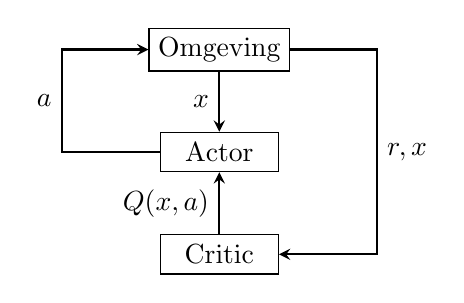
\begin{tikzpicture}[node distance=0.8cm, auto, >=latex']
        % Definieer stijlen voor verschillende soorten knooppunten
        \tikzstyle{startstop} = [rectangle, rounded corners, minimum width=1.5cm, minimum height=0.5cm,text centered, draw=black, fill=red!0]
        \tikzstyle{process} = [rectangle, minimum width=1.5cm, minimum height=0.5cm, text centered, draw=black, fill=orange!0]
        \tikzstyle{decision} = [rectangle, minimum width=1.5cm, minimum height=0.5cm, text centered, draw=black, fill=green!0]
        \tikzstyle{arrow} = [thick,->,>=stealth]

        % Knopen plaatsen
        \node (env) [process] {Omgeving};
        \node (act) [process, below of=env, yshift=-0.5cm] {Actor};
        \node (cri) [process, below of=act, yshift=-0.5cm] {Critic};

        % Pijlen tekenen
        \draw [arrow] (env) -- node[left] {$x$} (act);
        \draw [arrow] (cri) -- node[left] {$Q(x,a)$} (act);
        \draw [arrow] (env) -| ++(2,0) |- node[pos=0.25, right] {$r, x$} (cri);
        \draw [arrow] (act) -| ++(-2,0) |- node[pos=0.25, left] {$a$} (env);

    \end{tikzpicture}
    \caption{Flowchart van het Actor Critic model.}
    \label{fig:actorCriticFlowchart}
\end{figure}

Een belangrijk voordeel van dit model is dat het geschikt is voor zowel
discrete als continue actieruimten. Dit maakt het toepasbaar op veel
verschillende problemen, van spellen tot robotica. Het Actor-Critic-model
reduceert de variantie doordat de Critic een schatting maakt van de Q-functie.
Dit zorgt voor een stabieler en robuuster leerproces, vooral in spellen met
hoog-dimensionale toestandsruimten.

Een ander voordeel van het Actor-Critic-model is dat het een gelijktijdige
optimalisatie van het beleid en de waardefunctie mogelijk maakt. Bij DQN wordt
het beleid indirect geoptimaliseerd door een $\epsilon$-greedy-strategie. In
tegenstelling hiermee leert de Actor in het Actor-Critic-model met
exploratieruis, wat leidt tot snellere en efficiëntere convergentie, vooral in
situaties waarin een meer deterministisch beleid gewenst is.

\subsection{Proces}
Het DDPG-algoritme, zoals weergegeven in Algoritme \ref{alg:ddpg}, begint met
de initialisatie van het Actor-netwerk, het target Actor-netwerk, het
Critic-netwerk, het target Critic-netwerk en de replay buffer. Tijdens elke
episode genereert het algoritme exploratieruis op basis van een
Ornstein-Uhlenbeck-ruisproces, dat wordt gebruikt om te bepalen of de agent
kiest voor exploratie of exploitatie. De actieselectie wordt uitgevoerd door
het Actor-netwerk, waarbij exploratieruis wordt toegevoegd om voldoende
exploratie te waarborgen.

Het leerproces omvat het samplen van willekeurige minibatches uit de replay
buffer, het berekenen van doelwaarden en het updaten van zowel het Critic- als
het Actor-netwerk. Hierbij wordt gebruikgemaakt van policy gradients en een
soft update van de doelnetwerken. Dit draagt bij aan een stabiele optimalisatie
van het beleid. -
\begin{algorithm}[h]
    \caption{DDPG-algoritme \cite{ddpg} \label{alg:ddpg}}
    \begin{algorithmic}
        \State Initialiseer willekeurig het critic-netwerk $Q(s, a | \theta^Q)$ en het actor-netwerk
        $\mu(s | \theta^{\mu})$ met gewichten $\theta^{Q}$ en $\theta^{\mu}$.
        \State Initialiseer het target netwerk $Q'$ en $\mu'$ met gewichten $\theta^{Q'}
            \leftarrow \theta^{Q}$, $\theta^{\mu'} \leftarrow \theta^{\mu}$
        \State Initialiseer de replay buffer $R$
        \For{episode = 1, M}
        \State Initialiseer een willekeurig proces $\mathcal{N}$ voor actie-exploratie
        \State Ontvang de initiële waarnemingsstatus $s_1$
        \For{t = 1, T}
        \State Selecteer actie $a_t = \mu(s_t | \theta^{\mu}) + \mathcal{N}_t$
        volgens het huidige beleid en exploratieruis
        \State Voer actie $a_t$ uit en observeer beloning $r_t$ en nieuwe status $s_{t+1}$
        \State Sla de transitie $(s_t, a_t, r_t, s_{t+1})$ op in $R$
        \State Neem een willekeurige minibatch van $N$ transities $(s_i, a_i, r_i, s_{i+1})$ uit $R$
        \State Bereken:
        \begin{equation}
            y_i = r_i + \gamma Q'(s_{i+1}, \mu'(s_{i+1} | \theta^{\mu'}) | \theta^{Q'})
        \end{equation}

        \State Update de critic door de volgende verliesfunctie te minimaliseren:
        \begin{equation}
            L = \frac{1}{N} \sum_i (y_i - Q(s_i, a_i | \theta^Q))^2
        \end{equation}
        \State Update de actor-policy met behulp van de volgende policy-gradient:
        \begin{equation}
            \nabla_{\theta^{\mu}} J \approx
            \frac{1}{N} \sum_i
            \nabla_{a} Q(s, a | \theta^Q)|_{s = s_i, a = \mu(s_i)}
            \nabla_{\theta^\mu} \mu(s | \theta^\mu)|_{s_i}
        \end{equation}
        \State Update de targetnetwerken:
        \begin{equation}
            \theta^{Q'} \leftarrow \tau \theta^{Q} + (1 - \tau) \theta^{Q'}
        \end{equation}
        \begin{equation}
            \theta^{\mu'} \leftarrow \tau \theta^{\mu} + (1 - \tau) \theta^{\mu'}
        \end{equation}
        \EndFor
        \EndFor
    \end{algorithmic}
\end{algorithm}

\subsection{Toepassingen}
De flexibiliteit en kracht van DDPG maken het geschikt voor een breed scala aan
toepassingen, variërend van robotbesturing en autonome systemen tot complexe
simulatieomgevingen. Door zijn vermogen om te leren in continue actieruimtes
onderscheidt DDPG zich als een veelbelovende methode voor geavanceerde
reinforcement learning-uitdagingen.

\chapter{Kenmerken van specifieke Computerspellen}
Er zijn talloze computerspellen met diverse en uitdagende omgevingen voor de
toepassing van reinforcement learning (RL)-algoritmes. Spellen kunnen sterk van
elkaar verschillen in aspecten zoals structuur, dynamiek, complexiteit en
speeltijd. Al deze aspecten kunnen dergelijke invloed hebben op de
effectiviteit van RL-algoritmes. Elk type spel stelt specifieke eisen aan een
RL-algoritme, afhankelijk van aspecten zoals de omvang van de toestandsruimte,
de regels en beperkingen, en de vereiste strategische vaardigheden.

In dit hoofdstuk worden de specifieke kenmerken van vier computerspellen met
elkaar vergeleken: een \textit{auto-racespel} waar de agent het
autobesturingssysteem is, \textit{Snake} waar de agent de slang is,
\textit{Schaken} waar de agent de schaker is en \textit{Super Mario Bros} waar
de agent Mario is. Een overzicht van alle speleigenschappen is te zien in Tabel
??.

\section{Indeling en Strategische Diepgang van Spellen} Spellen kunnen worden ingedeeld op basis van hun genre en de mate van
strategische diepgang die nodig is om succesvol te zijn. Actie- en
platformspellen, zoals \textit{Super Mario Bros}, hebben een gemiddelde
strategische diepgang. Het doel is obstakels te overwinnen, vijanden te
ontwijken of verslaan en tegelijkertijd gouden munten te verzamelen. Dit soort
spellen vereist doorgaans korte termijn optimalisatie en directe reacties.

Strategiespellen, zoals \textit{Schaken}, vragen daarentegen om diepgaande
planning en vooruitdenken. Hier moet een speler of agent een reeks mogelijke
toekomstige toestanden analyseren en anticiperen op de acties van een
tegenstander. De strategische diepgang maakt leren complex, omdat beloningen
vaak cumulatief en pas aan het einde van het spel duidelijk worden. Dergelijke
spellen vereisen geavanceerde reinforcement learning (RL)-algoritmes die
langetermijnplanning ondersteunen.

Puzzel-/actiespellen, zoals \textit{Snake}, zijn minder afhankelijk van
strategie. Hier draait het om patroonherkenning en korte termijn optimalisatie,
waarbij eenvoudige RL-algoritmes voldoende zijn om succesvol te leren. Het doel
is bijvoorbeeld appels te verzamelen zonder jezelf te raken, waarbij de
beloningsstructuur rechtlijnig is.

Simulatie- en racegames, zoals een racespel met een zelfrijdende auto, richten
zich op efficiënt en veilig navigeren over een parcours. Hier ligt de nadruk op
het optimaliseren van gedrag in een gesimuleerde omgeving, vaak zonder de
noodzaak van complexe planningsstrategieën.

Deze variatie in genres en strategische eisen bepaalt welk type RL-algoritme
het meest geschikt is voor een spel. Complexere spellen met hogere strategische
diepgang vereisen geavanceerdere algoritmes, terwijl eenvoudigere spellen vaak
volstaan met directe responsmechanismen.

\section{Indeling van Spellen}
\textit{Super Mario Bros} valt binnen het genre van actie- en platformspellen. Het doel van het spel is over hindernissen springen en vijanden te ontwijken en verslaan en tegelijkertijd gouden munten te verzamelen. \textit{Schaken} daarentegen is een strategiespel, dat volledig turn-based is en gericht op denkvermogen, vooruitdenken en strategische planning. \textit{Snake} wordt vaak als een puzzel-/actiespel beschouwd, waarbij het doel is een appel te eten terwijl je niet jezelf raakt; hier is patroonherkenning belangrijk. Een zelfrijdende auto in een racespel valt binnen het genre van simulatie en racegames. Het draait om het efficiënt en veilig navigeren over een parcours. Dit wordt vaak gebruikt bij offline racespellen waar je tegen de computer speelt.

\section{Strategische Diepgang}
De mate van strategische diepgang in een spel is een van de belangrijkste
factoren die bepalen welk type RL-algoritme geschikt is. Strategie verwijst
naar het vermogen om vooruit te denken en acties te plannen die op lange
termijn voordelig zijn. Dit varieert sterk tussen spellen.

Strategische spellen, zoals \textit{Schaken}, vereisen dat een agent ver
vooruit denkt en een reeks mogelijke toekomstige toestanden analyseert. Hier is
langetermijnplanning essentieel. De agent moet niet alleen rekening houden met
de huidige toestand, maar ook anticiperen op de mogelijke acties van een
tegenstander en de daaropvolgende uitkomsten. Bij strategische spellen is het
leren complex, omdat beloningen vaak cumulatief en pas aan het einde van het
spel duidelijk worden.

Aan de andere kant zijn er spellen zoals \textit{Snake}, waarin strategie een
veel minder belangrijke rol speelt. In deze spellen zijn acties vaak gebaseerd
op eenvoudige regels en is de beste keuze meestal direct duidelijk. Het succes
van een speler hangt hier voornamelijk af van korte termijn optimalisatie.
Dergelijke spellen vereisen relatief eenvoudige RL-algoritmes, die zijn
ontworpen om direct te reageren op beloningen of straffen zonder complexe
planningsstrategieën. De eenvoudige structuur en beloningsmechanismen maken het
leerproces rechtlijnig en efficiënt.

\section{Beslissingsdynamiek en Tijdgevoeligheid}
De snelheid waarmee de omgeving van een spel verandert, bepaalt in grote mate
hoe moeilijk het is voor een RL-agent om effectief te leren en te reageren.

De beslissingsdynamiek verschilt sterk tussen de spellen. \textit{Super Mario
    Bros} vereist snelle real-time beslissingen. De agent moet op het juiste moment
springen of een vijand ontwijken, en timing is hierbij cruciaal. Bij
\textit{Schaken} is er juist geen tijdsdruk; de agent kan lang “nadenken” over
elke zet. \textit{Snake} zit er tussenin: hoewel het spel niet zo snel is als
\textit{Mario}, zit er wel een kleine tijdsdruk achter, maar dit is meestal
verwaarloosbaar. Timing en patroonherkenning worden belangrijker naarmate het
spel vordert. Bij een zelfrijdende auto in een racespel ligt de
beslissingsdynamiek real-time. Hier zijn snelheid en precisie van beslissingen
belangrijk, omdat milliseconden het verschil kunnen maken tussen een
succesvolle race en een botsing.

\section{Complexiteit}
De complexiteit van de regels en doelen varieert sterk. \textit{Super Mario
    Bros} heeft relatief eenvoudige regels: de agent moet vijanden vermijden en
verslaan, munten verzamelen, en het einde van het level bereiken. De
complexiteit van de vijanden en het terrein neemt echter toe naarmate de levels
moeilijker worden. \textit{Schaken} heeft relatief eenvoudige basisregels: zes
verschillende stukken met elk unieke bewegingsmogelijkheden. Het doel, het
schaakmat zetten van de tegenstander, vereist echter strategisch inzicht en
planning. Dit maakt \textit{Schaken} bijzonder uitdagend voor een RL-agent
vanwege de enorme toestandsruimte en de langetermijnplanning die nodig is.
\textit{Snake} heeft zeer eenvoudige regels: de agent moet voedsel verzamelen
en mag niet botsen met de muur of zichzelf. De uitdaging ligt in de toenemende
snelheid en lengte van de slang. Een zelfrijdende auto in een racespel heeft
daarentegen te maken met complexe regels die gebaseerd zijn op realistische
fysica. Het doel is simpel: zo snel mogelijk de finish bereiken.

\subsection{Regels en Beperkingen}
De complexiteit en het aantal regels in een spel spelen een cruciale rol in de
uitdaging die een RL-agent tegenkomt.

\subsubsection{Spellen met veel regels en vaste patronen}
Spellen zoals 4-op-een-rij of boter-kaas-en-eieren hebben een voorspelbare
structuur en strikte regels. De mogelijke zetten en uitkomsten zijn beperkt,
wat het spel eenvoudiger maakt om te modelleren. RL-algoritmes kunnen hier
profiteren van waarschijnlijkheidsmodellen en gestructureerde planning. De
voorspelbaarheid van deze spellen vermindert de onzekerheid in het leerproces.
Een RL-agent kan relatief eenvoudig een optimale strategie leren door alle
mogelijke acties te analyseren en te kiezen voor de meest belonende uitkomst.

\subsubsection{Spellen met weinig regels en veel vrijheid}
Spellen zoals GTA of Call of Duty bieden een grote mate van keuzevrijheid. De
speler kan vrij bewegen in een open wereld, interacties aangaan en talloze
acties uitvoeren. Deze spellen hebben een enorme toestandsruimte, die
driedimensionaal en dynamisch is. Dergelijke spellen vereisen een flexibel en
adaptief RL-algoritme. Het is onrealistisch voor een RL-agent om alle mogelijke
acties en toestanden volledig te doorzoeken. Algoritmes zoals Proximal Policy
Optimization (PPO) zijn hier geschikt. PPO gebruikt stochastische
beleidsmodellen en leert door te experimenteren met acties, waarbij het snel
aanpassingen kan maken op basis van feedback.

\section{Dynamiek en Tijdgevoeligheid}
De snelheid waarmee de omgeving van een spel verandert, bepaalt in grote mate
hoe moeilijk het is voor een RL-agent om effectief te leren en te reageren.

\subsection{Turn-based spellen}
Spellen zoals \textit{Schaken} of Monopoly bieden de speler voldoende tijd om
de optimale actie te berekenen. Omdat de omgeving niet continu verandert, kan
een RL-algoritme worden ingezet om een uitgebreide analyse te maken van alle
mogelijke uitkomsten van een actie. Dit type algoritme is bijzonder effectief
in spellen waar de agent kan profiteren van gestructureerde planning en
voorspelbare omgevingen.

\subsection{Realtime spellen}
In spellen zoals \textit{Mario Bros} of Tetris veranderen de omstandigheden
continu. Obstakels bewegen, vijanden verschijnen en de tijdsdruk vereist snelle
besluitvorming. Voor deze spellen zijn algoritmes nodig die snel leren en
direct reageren, met neurale netwerken, waardoor het algoritme in real-time
beslissingen kan nemen op basis van eerdere ervaringen.

\section{Beloningsstructuur}
Beloningen vormen de kern van RL en bepalen hoe een agent leert. De manier
waarop beloningen worden toegekend, varieert sterk tussen spellen.

\subsection{Directe beloningen}
Spellen zoals \textit{Snake} bieden onmiddellijke feedback. Elke actie
resulteert direct in een beloning (zoals punten voor het eten van voedsel) of
een straf (zoals botsingen). RL-algoritmes die afhankelijk zijn van directe
beloningen werken goed in deze context, omdat ze snel leren welke acties
voordelig zijn.

\subsection{Cumulatieve beloningen}
In strategische spellen zoals \textit{Schaken} worden beloningen vaak pas aan
het einde van het spel toegekend. Dit vereist dat de agent leert om acties te
nemen die op lange termijn voordelig zijn. Het leren wordt complexer omdat de
agent beloningen moet toeschrijven aan acties die mogelijk vele stappen eerder
werden ondernomen.

\chapter{De invloed van spelkenmerken  op Reinforcement Learning-Algoritmes}

\section{Strategische Diepgang}
\subsection*{Q-Learning:}
Q-Learning presteert goed in spellen met een lage strategische diepgang, zoals
Snake. Omdat Q-Learning gebruikmaakt van een Q-tabel die alleen de waarde van
elke toestand-actiecombinatie opslaat. Wat het niet geschikt maakt voor spellen
met een grote toestandsruimte of langetermijnstrategieën, zoals Schaken.

\subsection*{DQN:}
DQN breidt Q-Learning uit door neurale netwerken te gebruiken om Q-waarden te
benaderen, wat het geschikter maakt voor spellen met een gemiddelde
strategische diepgang, zoals Mario Bros. Het algoritme kan leren van zowel
directe- als kortetermijnfeedback, maar mist de meer geavanceerde planning die
nodig zijn voor spellen die een diepere strategie gebruiken.

\subsection*{DDPG:}
DDPG is gericht op continue actieruimtes en wordt minder beïnvloed door de
strategische diepgang, maar eerder door de mate waarin de acties moeten worden
afgestemd. Voor spellen zoals Mario Bros, waar timing en actiecontrole
belangrijk zijn, kan DDPG strategieën leren door zowel korte- als
langetermijnfeedback te gebruiken.

\section{Regels en Beperkingen}
\subsection*{Q-Learning:}
Werkt het beste in spellen met eenvoudige regels en beperkte keuzevrijheid,
zoals Snake. Door de vaste en voorspelbare omgeving kunnen de toestands- en
actieruimtes volledig worden doorzocht, wat het leren relatief eenvoudig maakt.

\subsection*{DQN:}
Presteert goed in spellen met relatief meer complexiteit in regels, zoals Mario
Bros. Door het gebruik van neurale netwerken kan het algoritme generalisaties
maken, waardoor het beter omgaat met spellen met grotere toestandsruimtes en
variabele regels.

\subsection*{DDPG:}
Bij spellen met een hoge keuzevrijheid, zoals een racespel, is DDPG beter in
staat om acties nauwkeurig af te stemmen op een veranderende toestandsruimte.
De flexibiliteit van DDPG maakt het een betere keuze voor omgevingen zonder
strikte beperkingen.

\section{Dynamiek en Tijdgevoeligheid}
\subsection*{Q-Learning:}
Het algoritme is minder geschikt voor real-time spellen vanwege zijn
tabelgebaseerde aanpak. Voor spellen zoals Snake met beperkte snelheid en
eenvoudige dynamiek kan Q-Learning goed werken. Het heeft moeite met een snel
veranderende omgeving.

\subsection*{DQN:}
Werkt goed in real-time dynamische spellen zoals Mario Bros. Door gebruik te
maken van neurale netwerken en technieken zoals experience replay, kan DQN
beter omgaan met snelle veranderingen en real-time beslissingen.

\subsection*{DDPG:}
DDPG is bij het best geschikt voor dynamische spellen waar continue aanpassing
bij nodig is, zoals een racespel of geavanceerde spellen. Het algoritme
combineert actie-optimalisatie met de snelheid van beleidsupdates. Dit maakt
het effectief in real-time situaties.

\section{Beloningsstructuur}
\subsection*{Q-Learning:}
Werkt goed met directe beloningen, zoals in Snake. Omdat Q-Learning beloningen
koppelt aan toestands-actiecombinaties, leert het snel in omgevingen waar
feedback direct vergeven wordt.

\subsection*{DQN:}
Kan omgaan met zowel directe als cumulatieve beloningen, zoals in Mario Bros.
Het algoritme gebruikt de neurale netwerken om toekomstige beloningen te
voorspellen, wat helpt bij het optimaliseren van zowel kortetermijn- als
langetermijnacties.

\subsection*{DDPG:}
Presteert beter in omgevingen met cumulatieve beloningen, zoals een complexe
racespelomgeving. Het algoritme gebruikt de Actor-Critic-structuur om
beloningen over langere tijd te maximaliseren en leert efficiënter in
omgevingen met variabele beloningsstructuren.

\section{Complexiteit van de Toestandsruimte}
\subsection*{Q-Learning:}
Functioneert alleen in spellen met een kleine toestandsruimte, zoals Snake.
Omdat Q-Learning expliciet een Q-tabel opbouwt, wordt het onpraktisch voor
spellen met grote toestandsruimtes, zoals Schaken of Mario Bros.

\subsection*{DQN:}
Kan omgaan met grotere toestandsruimtes dankzij het gebruik van neurale
netwerken. Voor spellen zoals Mario Bros kan DQN gemakkelijker leren door
patronen te herkennen en te generaliseren, zonder afhankelijk te zijn van een
volledige tabel.

\subsection*{DDPG:}
Geschikt voor spellen met grote toestandsruimtes en continue actieruimtes. In
moeilijke omgevingen zoals simulaties kan DDPG strategieën leren door
geavanceerde Actor-Critic-modellen, wat schaalbaarheid mogelijk maakt.

\section{Onvoorspelbaarheid}
\subsection*{Q-Learning:}
Is niet goed bestand tegen onvoorspelbaarheid. Het algoritme werkt het beste in
deterministische omgevingen waar de uitkomsten van acties bekend en consistent
zijn, zoals Snake.

\subsection*{DQN:}
Kan omgaan met enige onvoorspelbaarheid, zoals in Mario Bros, door gebruik te
maken van schattingen en neurale netwerken om patronen te herkennen en aan te
passen.

\subsection*{DDPG:}
Presteert het best in omgevingen met een hoge mate van onvoorspelbaarheid. Het
algoritme past zich continu aan dankzij de Actor-Critic-structuur, wat het
beter maakt in dynamische omgevingen waar acties verschillende eindresultaten
kunnen opleveren.

\chapter{Onderzoeksmethoden}
In dit onderzoek bekijken we hoe goed verschillende reinforcement
learning-algoritmes werken bij het spelen van computerspellen. We onderzoeken
drie algoritmes: Q-Learning, Deep Q-Network (DQN) en Deep Deterministic Policy
Gradient (DDPG). Deze drie zijn gekozen omdat ze samen een goed beeld geven van
eenvoudige tot meer ingewikkelde methoden binnen reinforcement learning. We
testen deze algorithme op het spel snake.

\section{Technische Uitvoering}
We hebben alle testen uitgevoerd met Python 3.8 \cite{python_docs} als
programmeertaal. Voor het maken van de neurale netwerken gebruikten we PyTorch
\cite{pytorch_docs}. De spelomgevingen hebben we gemaakt met Pygame
\cite{pygame}. Voor het verwerken van getallen en het maken van grafieken
gebruikten we NumPy \cite{numpy_docs} en Matplotlib \cite{matplotlib_docs}.

\section{Verzamelen van Gegevens}
We hebben verschillende metingen gedaan om te zien hoe goed de algoritmes
werken. We keken naar de gemiddelde score per speelronde, hoe lang het duurde
voordat het algoritme het spel onder de knie had, en hoe stabiel de prestaties
waren. Deze gegevens verzamelden we over 10.000 speelrondes.Om zeker te zijn
van onze resultaten hebben we elk experiment vijf keer uitgevoerd.

\section{Optimalisatie van Instellingen}
Voor elk algoritme hebben we systematisch gezocht naar de beste
hyperparameters. We testten verschillende waardes voor de leersnelheid, hoe
belangrijk toekomstige beloningen zijn, en hoe vaak het algoritme nieuwe dingen
moest proberen. Deze instellingen hebben we voor elk spel apart bepaald.

\chapter{Logboek}
\small
\section*{Groepsactiviteiten}
\begin{longtable}{|p{0.15\textwidth}|p{0.1\textwidth}|p{0.1\textwidth}|p{0.55\textwidth}|}
    \hline
    \textbf{Datum} & \textbf{Tijd} & \textbf{Plaats} & \textbf{Activiteiten + Resultaten}                                                                                                                                                                                                                                                                                   \\
    \hline
    02-07-2024     & 3 uur         & School          & Onderzoek over AI, we leerden alle drie over reinforced learning, wat die inhield en wat we interessant vonden. PWS presentatie, deze heeft goed geholpen om te begrijpen wat we moeten doen. De bronnenlijst is gemaakt, deze duurt het langst. Hier zijn de bronnen ingezet waarvan wij denken dat ze handig zijn. \\
    \hline
    28/08/2024     & 1 uur         & School          & Overleg tijdens les                                                                                                                                                                                                                                                                                                  \\
    \hline
    04/09/2024     & 1 uur         & School          & Overleg tijdens les en taakverdeling gedeeltelijk geregeld                                                                                                                                                                                                                                                           \\
    \hline
    11/09/2024     & 1 uur         & School          & Inlezen onderwerp                                                                                                                                                                                                                                                                                                    \\
    \hline
    25/09/2024     & 1 uur         & School          & Overleg indeling schrijven                                                                                                                                                                                                                                                                                           \\
    \hline
    04/09/2024     & 1 uur 15 min  & School          & Inlezen onderwerp. Onderling plan van aanpak besproken                                                                                                                                                                                                                                                               \\
    \hline
    11/09/2024     & 1 uur         & School          & Taken en deadlines besproken. Taken verdeeld voor volgende pws uur. Verder ingelezen over onderwerp                                                                                                                                                                                                                  \\
    \hline
    02/10/2024     & 1 uur         & School          & Bronnenlijst overleg                                                                                                                                                                                                                                                                                                 \\
    \hline
    09/10/2024     & 1 uur         & School          & Voorwoord maken                                                                                                                                                                                                                                                                                                      \\
    \hline
    16/10/2024     & 1 uur         & School          & Onderzoek AI                                                                                                                                                                                                                                                                                                         \\
    \hline
    23/10/2024     & 1 uur         & School          & Onderzoek RL                                                                                                                                                                                                                                                                                                         \\
    \hline
    06/11/2024     & 1 uur         & School          & Inlezen                                                                                                                                                                                                                                                                                                              \\
    \hline
    13/11/2024     & 1 uur         & School          & Verder inlezen                                                                                                                                                                                                                                                                                                       \\
    \hline
    20/11/2024     & 1 uur         & School          & Layout maken                                                                                                                                                                                                                                                                                                         \\
    \hline
    27/11/2024     & 1 uur         & School          & Meer samenvatten                                                                                                                                                                                                                                                                                                     \\
    \hline
    04/12/2024     & 1 uur         & School          & Overleg                                                                                                                                                                                                                                                                                                              \\
    \hline
\end{longtable}
\newpage
\section*{Matthijs}
\begin{longtable}{|p{0.15\textwidth}|p{0.1\textwidth}|p{0.1\textwidth}|p{0.55\textwidth}|}
    \hline
    \textbf{Datum} & \textbf{Tijd} & \textbf{Plaats}         & \textbf{Activiteiten + Resultaten}                                                                                                                                                                                                                                  \\
    \hline
    06-07-2024     & 1 uur         & Thuis                   & Eerste Stanfords CS234 college bekeken uit de winter van 2019 \cite{stanford_cs234}. Het kopje Definitie van Reinforcement Learning geschreven. (Later besloten dit in de inleiding te zetten)                                                                      \\
    \hline
    29/07/2024     & 3 uur         & Thuis                   & Snake spel geschreven in python en github aangemaakt en begonnen met Q-learning te implementeren \cite{snake_game} \cite{python_docs}                                                                                                                               \\
    \hline
    30/07/2024     & 2 uur         & Thuis                   & Q-learning geïmplementeerd. Maar de agent leert nog slecht.                                                                                                                                                                                                         \\
    \hline
    31/07/2024     & 3 uur         & Thuis                   & Q-learning hyperparameters uitgetest en optimale gevonden.                                                                                                                                                                                                          \\
    \hline
    03/08/2024     & 2 uur         & Thuis                   & Kennis opgedaan over machine learning en andere types dan reinforcement learning en hoe het verschilt van super- en unsupervised learning \cite{ml_types}                                                                                                           \\
    \hline
    05/08/2024     & 3 uur         & Thuis                   & Begin gemaakt een theoretisch kader \cite{spinning_up}                                                                                                                                                                                                              \\
    \hline
    06/08/2024     & 2 uur         & Thuis                   & Theoretisch kader afgemaakt.                                                                                                                                                                                                                                        \\
    \hline
    08/08/2024     & 2 uur         & Thuis                   & LaTeX geleerd en eerste layout gemaakt van het PWS met alle kopjes.                                                                                                                                                                                                 \\
    \hline
    1/09/2024      & 3 uur         & Thuis                   & Voorstel gemaakt                                                                                                                                                                                                                                                    \\
    \hline
    10/09/2024     & 3 uur         & Thuis, online met groep & Voorwoord gemaakt, overleg over de aanpak en het algemene idee.                                                                                                                                                                                                     \\
    \hline
    20/09/2024     & 2 uur         & Thuis                   & Het Q-learning algoritme tijdsefficiënter gemaakt met numpy en een bug gefixt in snake zodat er nu geen appel kan spawnen in de slang zelf \cite{numpy_docs}                                                                                                        \\
    \hline
    27/09/2024     & 4 uur         & Thuis                   & Script gemaakt voor resultaten van Q-learning in grafiek (5000 woorden, gebruik van Matplotlib). Hyperparameters uitgetest en optimale gevonden. Elke training kostte ongeveer 15 minuten. (gemiddeld score van beste waardes was 60 appels) \cite{matplotlib_docs} \\
    \hline
    24/10/2024     & 4 uur         & Thuis                   & Script gemaakt voor DQN algoritme met PyTorch \cite{pytorch_docs} \cite{pytorch_rl}                                                                                                                                                                                 \\
    \hline
    17/11/2024     & 3 uur         & Thuis                   & Hoofdstuk Kenmerken van specifieke algoritmes begonnen. Introductie geschreven en DQN Algoritme vertaald \cite{delayed_rewards} \cite{multi_agent_rl}                                                                                                               \\
    \hline
    24/11/2024     & 3 uur         & Thuis                   & Sectie Deep Q-Network begonnen. Algoritme vertaald, proces beschreven \cite{dqn_nature}                                                                                                                                                                             \\
    \hline
    28/11/2024     & 1 uur         & Thuis                   & Flowchart van Deep Q-Network algoritme gemaakt en verder geschreven                                                                                                                                                                                                 \\
    \hline
    29/11/2024     & 3 uur         & Thuis                   & Kopje Neuraal Netwerk geschreven en diagram van neuraal netwerk in DQN gemaakt \cite{nn_math}                                                                                                                                                                       \\
    \hline
    31/11/2024     & 3 uur         & Thuis                   & Onderzoek over Deep Deterministic Policy Gradient en algoritme vertaald \cite{ddpg} \cite{silver_dpg}                                                                                                                                                               \\
    \hline
    2/12/2024      & 2 uur         & Thuis                   & Proces van DDPG geschreven.                                                                                                                                                                                                                                         \\
    \hline
    3/12/2024      & 2 uur         & Thuis                   & Actor-Critic model geschreven en figuur Flowchart van Actor Critic model gemaakt en Toepassingen geschreven.                                                                                                                                                        \\
    \hline
    4/12/2024      & 2 uur         & Thuis                   & Onderzoeksmethoden geschreven.                                                                                                                                                                                                                                      \\
    \hline
    5/12/2024      & 1 uur         & Thuis                   & Puntes op de i gezet.                                                                                                                                                                                                                                               \\
    \hline
\end{longtable}

\section*{Thom}
\begin{longtable}{|p{0.15\textwidth}|p{0.1\textwidth}|p{0.1\textwidth}|p{0.55\textwidth}|}
    \hline
    \textbf{Datum} & \textbf{Tijd} & \textbf{Plaats}         & \textbf{Activiteiten + Resultaten}                             \\
    \hline
    03/09/2024     & 2 uur         & Thuis                   & Inlezen over het onderwerp \cite{wiki_rl}                      \\
    \hline
    04/09/2024     & 2 uur         & Thuis                   & Inlezen over het onderwerp \cite{scribbr_rl}                   \\
    \hline
    05/09/2024     & 2 uur         & Thuis                   & Inlezen over het onderwerp \cite{geeksforgeeks_rl}             \\
    \hline
    06/09/2024     & 2 uur         & Thuis                   & Inlezen over het onderwerp \cite{oracle_rl}                    \\
    \hline
    10/09/2024     & 3 uur         & Thuis, online met groep & Voorwoord maken, overleg over het idee                         \\
    \hline
    26/09/2024     & 2,5 uur       & Thuis                   & Layout maken van het verslag, verder inlezen over onderwerp    \\
    \hline
    01/10/2024     & 3 uur         & Thuis                   & Matthijs' theoretisch kader verbeterd                          \\
    \hline
    02/10/2024     & 3 uur         & Thuis                   & Uitleg theoretisch kader                                       \\
    \hline
    04/10/2024     & 3 uur         & Thuis                   & Herschrijven theoretisch kader                                 \\
    \hline
    06/10/2024     & 2 uur         & Thuis                   & Antwoorden deelvraag 1                                         \\
    \hline
    07/10/2024     & 3 uur         & Bij pepijn              & Inleiding herschreven. Plan van aanpak gemaakt.                \\
    \hline
    08/11/2024     & 3 uur         & Thuis                   & Herschrijven van tekst / nalezen versie voor controle moment 2 \\
    \hline
    03/12/2024     & 3 uur         & Thuis                   & Afmaken plaatjes maken                                         \\
    \hline
    04/12/2024     & 2 uur         & Thuis                   & Afmaken PWS voor controlemoment                                \\
    \hline
    05/12/2024     & 2 uur         & Thuis                   & Puntjes op i zetten                                            \\
    \hline
\end{longtable}
\newpage
\section*{Pepijn}
\begin{longtable}{|p{0.15\textwidth}|p{0.1\textwidth}|p{0.1\textwidth}|p{0.55\textwidth}|}
    \hline
    \textbf{Datum} & \textbf{Tijd} & \textbf{Plaats}         & \textbf{Activiteiten + Resultaten}                                                                                         \\
    \hline
    30/08/2024     & 2 uur         & Thuis                   & Ingelezen onderwerp \cite{ai_basics} \cite{datacamp_ai}                                                                    \\
    \hline
    1/09/2024      & 1 uur         & Thuis                   & Onderzoeksplan en -overzicht gemaakt(van het voorstel)                                                                     \\
    \hline
    03/09/2024     & 3 uur         & Thuis                   & Ingelezen over het onderwerp \cite{analytics_vidhya_rl} \cite{rl_guide}                                                    \\
    \hline
    04/09/2024     & 1 uur         & Thuis                   & Inlezen over q-learning \cite{q_learning_tutorial}                                                                         \\
    \hline
    07/09/2024     & 3,5 uur       & Thuis                   & Inlezen over het onderwerp en Deep q learning \cite{dqn_guide} \cite{sutton_barto}                                         \\
    \hline
    9/09/2024      & 3 uur         & Thuis                   & Ingelezen over het onderwerp \cite{dqn_paper}                                                                              \\
    \hline
    10/09/2024     & 3 uur         & Thuis, online met groep & Voorwoord gemaakt, overleg over de aanpak en het algemene idee.                                                            \\
    \hline
    07/10/2024     & 3 uur         & Thuis                   & Inleiding herschreven en lay-out van andere delen van het pws verbeterd. Plan van aanpak gemaakt voor de rest van het pws. \\
    \hline
    26/09/2024     & 3 uur         & Thuis                   & Inlezen over speleigenschappen \cite{pmlr-v119-cobbe20a} en begonnnen met het schrijven van deelvraag 2.                   \\
    \hline
    29/10/2024     & 3 uur         & Thuis                   & Verder gewerkt aan deelvraag 2 en bijna volledig uitgewerkt                                                                \\
    \hline
    30/10/2024     & 3 uur         & Thuis                   & Deelvraag 2 afgeschreven                                                                                                   \\
    \hline
    1/11/2024      & 2 uur         & Thuis                   & Alles nagelezen wat tot nu toe was gemaakt en de lay-out erg verbeterd.                                                    \\
    \hline
    08/11/2024     & 3 uur         & bij Thom                & Herschrijven van tekst /nalezen versie voor controle moment 2                                                              \\
    \hline
    26/11/2024     & 0,5 uur       & Thuis                   & Inleiding anders verwoord en fouten uit het pws gehaald                                                                    \\
    \hline
    03/12/2024     & 3 uur         & Thuis                   & Begonnen met deelvraag 3                                                                                                   \\
    \hline
    04/12/2024     & 2 uur         & Thuis                   & Deelvraag 3 afgemaakt en verbeterd                                                                                         \\
    \hline
    05/12/2024     & 3 uur         & Thuis                   & PWS nagelezen spelling verbeterd bronnotatie geregeld en puntjes op de i gezet.                                            \\
    \hline
\end{longtable}

\printbibliography
\addcontentsline{toc}{chapter}{Bibliografie}

\end{document}
